\documentclass{article}
\usepackage{amssymb}
\usepackage{amsmath}
\usepackage{indentfirst}
\usepackage{graphicx}
\usepackage{listings}
\usepackage{color}
\usepackage{float}
\definecolor{dkgreen}{rgb}{0,0.6,0}
\definecolor{gray}{rgb}{0.5,0.5,0.5}
\definecolor{mauve}{rgb}{0.58,0,0.82}

\lstset{frame=tb,
	language=Python,
	aboveskip=3mm,
	belowskip=3mm,
	showstringspaces=false,
	columns=flexible,
	basicstyle={\small\ttfamily},
	numbers=none,
	numberstyle=\tiny\color{gray},
	keywordstyle=\color{blue},
	commentstyle=\color{dkgreen},
	stringstyle=\color{mauve},
	breaklines=true,
	breakatwhitespace=true,
	tabsize=3
}

\author{Fu Min \ \ 72677006}
   \title{SI 211: Numerical Analysis\\ Homework 3 }
   
\begin{document}
\maketitle
\noindent \textbf{Problem 1}. 
Write a computer code in JULIA, Matlab, Python, or C++, which returns a natural spline
that intepolates the function $f : [x_0; x_N] \longrightarrow R$ at the equidistant points\\
\begin{align*}
x_i &= x_0 + h_i \ with \ \ h = \frac{x_N - x_0}{N}
\end{align*}
\indent \textbf{Solution.}
\begin{lstlisting}
def natural_cubic_spline(n, x , a ):

A = np.zeros(n);
l = np.zeros(n+1)
c = np.zeros(n+1)
z = np.zeros(n+1)
u = np.zeros(n)
b = np.zeros(n)
d = np.zeros(n)
# Step 1
h = (x[n] - x[0])/n
# Step 2 
for i in range( 1 , n ):
A[i] =  3 * (a[i + 1] - a[i]) / h - 3 * (a[i] - a[i - 1]) / h 
# Step 3 
l[0] = 1
u[0] = 0
z[0] = 0
#Step 4 
for i in range( 1 , n ):
l[i] =  2 * (x[i + 1] - x[i - 1]) - h * u[i - 1] 
u[i] =  h / l[i]
z[i] = (A[i] - h * z[i - 1]) / l[i]
# step 5 
l[n] = 1
z[n] = 0
c[n] = 0
# Step 6 
for j in range(n):
c[n-1-j] = z[n-1-j] - u[n-1-j] * c[n-j];
b[n-1-j] = (a[n-j] - a[n-1-j]) / h - h * (c[n-j] + 2 * c[n-1-j]) / 3
d[n-1-j] = (c[n-j] - c[n-1-j]) / (3 * h)
    return b,c,d
    
def S(x,a,b,c,d,endx):
    return a + b*(x-endx) + c * (x-endx)**2 + d * (x - endx)**3
\end{lstlisting}  
    
     
\noindent \textbf{Problem 2}. Use your computer code from the first exercise in order to compute a natural spline of the
function
$$f(x) = \frac{1}{1 + x^2}$$
   
on the interval $[x_0; x_N] = [-5; 5]$. You may set $N = 10$. Plot the function $f$ as well as thenatural spline that interpolates $f$.\\
\textbf{Solution.}\\
Code :
 \begin{lstlisting}
def f1(x):
    return 1.0 / (1.0 + x**2)
#problem 2
x1 = np.arange(-5,6)
n1 = len(x1)-1
a1 = f1(x1)
xx1 = np.linspace(-5, 5, 100)
b1,c1,d1 = natural_cubic_spline(n1, x1 , a1)
# Plot
fig = plt.figure(1)
axes = fig.add_subplot(1, 1, 1)
axes.plot(x1, a1, 'ko',label="data")
axes.plot(xx1, f1(xx1), 'k',label="True $f(x)$")
for i in range(10):
xx = np.linspace(x1[i], x1[i+1], 50)
axes.plot(xx, S(xx,a1[i],b1[i],c1[i],d1[i],x1[i]),label="$S_{%s}(x)$" % i)
axes.set_title(" natural Cubic Splines - f(x) = $1/(1+x^2)$")
axes.set_xlabel("x")
axes.set_ylabel("y")
axes.set_xlim([-6.0, 6.0])
axes.set_ylim([0, 1.5])
axes.legend(loc = 0)
plt.show()

\end{lstlisting}     
The figure of  function f as well as the natural spline that interpolates f.

  \begin{figure}[H]            \centering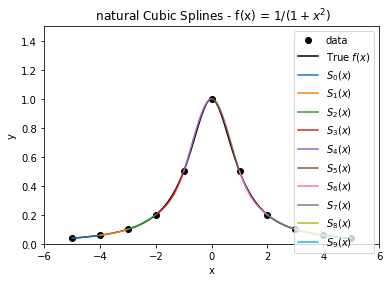
\includegraphics[width=3.5in,height=2.5in]{problem2.png}
	\caption{function f as well as the natural spline that interpolates f}
	\label{fig:graph}
  \end{figure}
\noindent \textbf{Problem 3}. Use your compute code to compute a natural spline of the function
$$f(x) = x^2$$
on the interval $[x0; xN] = [0; 1]$ with $x = 10$.What is the exact value for the integral
$$ \int_0^1 [f^{''}(x)]^2 dx = ? $$
Also compute the value 
$$ \int_0^1 [p{''}(x)]^2 dx = ? $$
for the interpolating spline. Explain how you compute this integral numerically. Which
value is bigger,$ \int_0^1 [f^{''}(x)]^2 dx  $ or $ \int_0^1 [p{''}(x)]^2 dx  ?$
\begin{lstlisting}
def f2(x):
   return x**2
#problem 3
x2 = np.arange(0,1.1,0.1)
n2 = len(x2)-1
a2 = f2(x2)
xx2 = np.linspace(0, 1, 100)
b2,c2,d2 = natural_cubic_spline(n2, x2 , a2)
# Plot
fig = plt.figure(2)
axes = fig.add_subplot(1, 1, 1)

axes.plot(x2, a2, 'ko',label="data")
axes.plot(xx2, f2(xx2), 'k',label="True $f(x)$")
for i in range(10):
xx = np.linspace(x2[i], x2[i+1], 50)
axes.plot(xx, S(xx,a2[i],b2[i],c2[i],d2[i],x2[i]),label="$S_{%s}(x)$" % i)
axes.set_title(" natural Cubic Splines - f(x) = $x^2$")
axes.set_xlabel("x")
axes.set_ylabel("y")
axes.set_xlim([0, 1])
axes.set_ylim([0, 1.5])
axes.legend(loc = 0)
plt.show()
\end{lstlisting}
The figure of  function f as well as the natural spline that interpolates f.

\begin{figure}[H]            \centering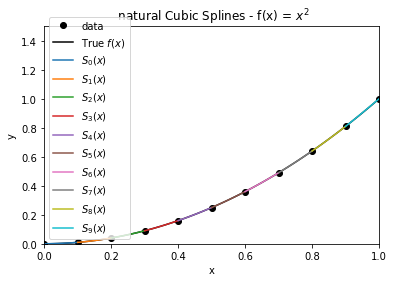
\includegraphics[width=3.5in,height=2.5in]{problem3.png}
	\caption{function f as well as the natural spline that interpolates f}
	\label{fig:graph}
\end{figure}
Because $f^{''}(x) = 2$,
$$ \int_0^1 |f^{''}(x)|^2 dx = \int_0^1 2^2 dx = 4 $$
And we have that\\	
	\begin{tabular}{cccccc}
		\hline
	    j &$x_j$&$a_j$&$b_j$&$c_j$&$d_j$\\
		\hline
	    0& 0  & 0   & 0.0577348& 0      & 4.22652\\
	    
	    1& 0.1& 0.01& 0.18453  & 1.26796&-1.1326\\
	    
	    2& 0.2& 0.04& 0.404144 & 0.928177&0.303867\\
	    
	  3& 0.3&0.09&   0.598895& 1.01934  &-0.0828729\\
	  
	    4& 0.4&0.16 &  0.800276& 0.994475&0.0276243\\
	    
	    5& 0.5&0.25&   1       & 1.00276&-0.0276243\\
	  
	    6& 0.6& 0.36&  1.19972 & 0.994475&0.0828729\\
	    
	    7& 0.7&0.49&   1.4011  &1.01934&-0.303867\\
	    
	    8& 0.8& 0.64&  1.59586 &0.928177&1.1326\\
	    
	    9& 0.9& 0.81&  1.81547 &1.26796&-4.22652\\
	    
        10& 1&  1   &          &        &  \\
		\hline
	\end{tabular}

$$ \int_0^1 |P^{''}(x)|^2 dx = \sum_{i = 0}^{9}\int_{x_i}^{x_{i+1}} |2c_i + 6*d_i(x-x_i)|^2 dx = 3.769$$
So
$ \int_0^1 [f^{''}(x)]^2 dx > \int_0^1 [p{''}(x)]^2 dx $.
\end{document} 